

\subsection{SPC evaluation}
\label{sec:eval_spc}
The evaluation section is now shifted to examine the images produced by the SPC. The images will be analyzed using the using a range of methods to examine the performance of the SPC. In this section the BRISQUE algorithm will be used again where connections to the previous result is drawn, a reconstructed image will be compared to an ideal image using homography, a set of images is presented reconstructed at different subsampling ratios, a edge response analysis i performed and the correlation between reconstruction performance and noise is conducted. 

\todo[inline]{The images captured was taken at a distance between 200 to 900 m}

\todo[inline]{List the specs?}

\subsubsection{Reconstructed performance Using reference image}
This evaluation is designed to get a measurement of expected image quality with the same metrics used in the synthetic case. As stated before, it is hard to obtain a reference image to the images produced by the SPC. One solution to obtain a reference image is to calculate a homography between images. But there are two problems of just performing a homography to obtain a reference image, the fist on is that, homography estimates the transformation between flat surfaces which excludes most natural images, and the second is that, the estimated homography will not be perfect an thus for example high contrast edges in the images will not match and then produce large errors in the performance measurements. To solve these two problems the scene is a flat surface with a printed pattern and to avoid the the error from sharp edges the pettern is constructed without any. To not complicate this experiment the reference image is the computer generated optimal images which is being transformed to fit the image captured by the SPC.\\[0.1in] 

The reference homography transformed image which was created using sine functions to avoid edges can be seen in figure~\ref{fig:hom_over_im} with the reconstructed images with different subsampling ratio.   


\begin{figure}[H]
    \centering
\begin{minipage}[h]{0.3\textwidth}
	\vspace*{1cm}
    
\includegraphics[width=1\textwidth]{result/hom/im_ref.png}
    \subcaption{Homography transformed refrence image}
    \label{fig:hom_ref}
\end{minipage}
\begin{minipage}[t]{0.22\textwidth}
    
\includegraphics[width = \textwidth]{result/hom/im_m5.png}
    \subcaption{5\%}
    \label{fig:hom_5}
    
\includegraphics[width = \textwidth]{result/hom/im_m20.png}
    \subcaption{20\%}
    \label{fig:hom_20}
\end{minipage}
\begin{minipage}[t]{0.22\textwidth}
    
\includegraphics[width = \textwidth]{result/hom/im_m10.png}
    \subcaption{10\%}
    \label{fig:hom_10}
    
\includegraphics[width = \textwidth]{result/hom/im_m25.png}
    \subcaption{25\%}
    \label{fig:hom_25}
\end{minipage}
\begin{minipage}[t]{0.22\textwidth}
    
\includegraphics[width = \textwidth]{result/hom/im_m15.png}
    \subcaption{15\%}
    \label{fig:hom_15}
    
\includegraphics[width = \textwidth]{result/hom/im_m30.png}
    \subcaption{30\%}
    \label{fig:hom_30}
\end{minipage}
    \caption{The reconstructed images with different number of measurements and the reference image transformed to fit the SPC images using homography.}
    \label{fig:hom_over_im}
\end{figure}

Before the results from the evaluation is presented it is worth noting that the reference image is a perfect simulated reference image, which was not effected by the uneven light source and quality of the print as the reconstructed image from the SPC, which for example can be seen in the edges of the reconstructed images in figure~\ref{fig:hom_5} to \ref{fig:hom_30}. In figure~\ref{fig:hom_score} below the same evaluation method as the reconstructed simulated images in section~\ref{sec:simulated_results} is used, PSNR and SSIM, because there is a reference image again. 


\begin{figure}[H]
    \centering
\begin{minipage}[t]{0.49\textwidth}
    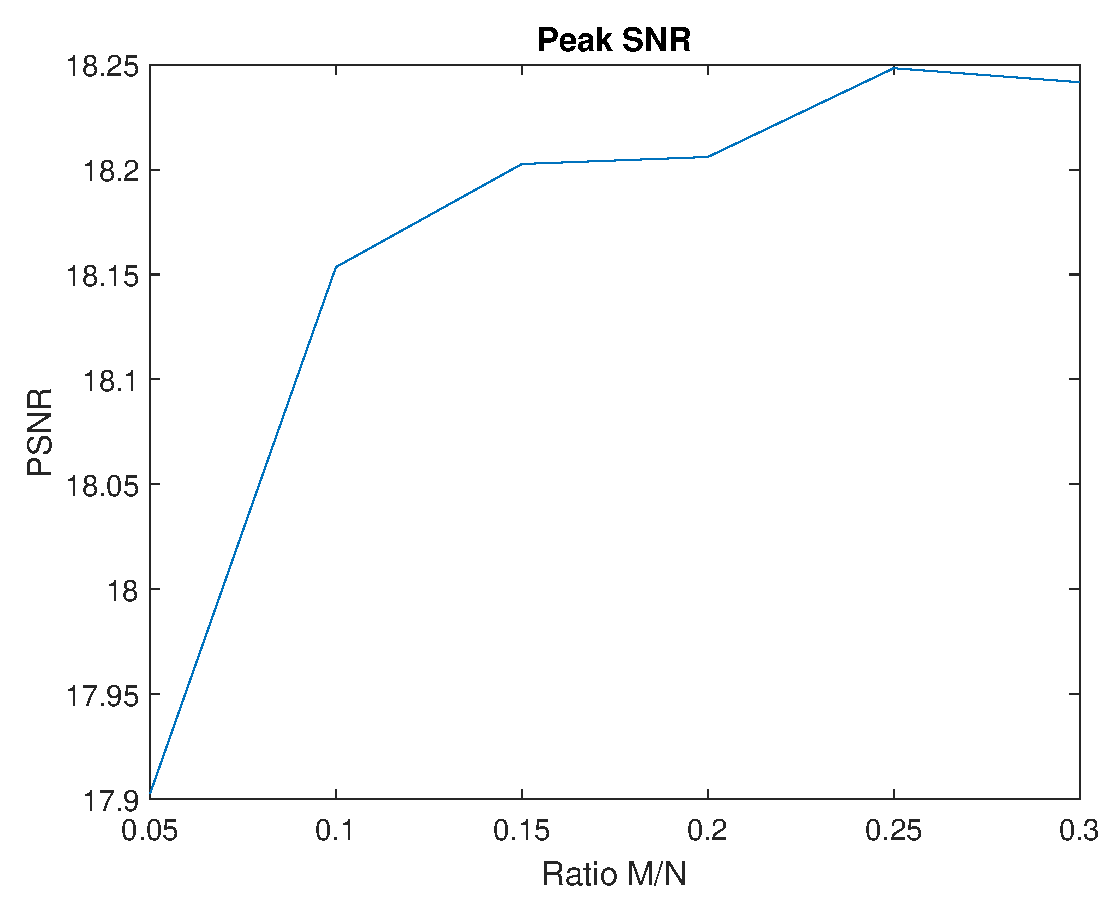
\includegraphics[width=1\textwidth]{result/homo/PSNR_2.eps}
    \subcaption{}
    \label{fig:hom_psnr}
\end{minipage}
\begin{minipage}[t]{0.49\textwidth}
    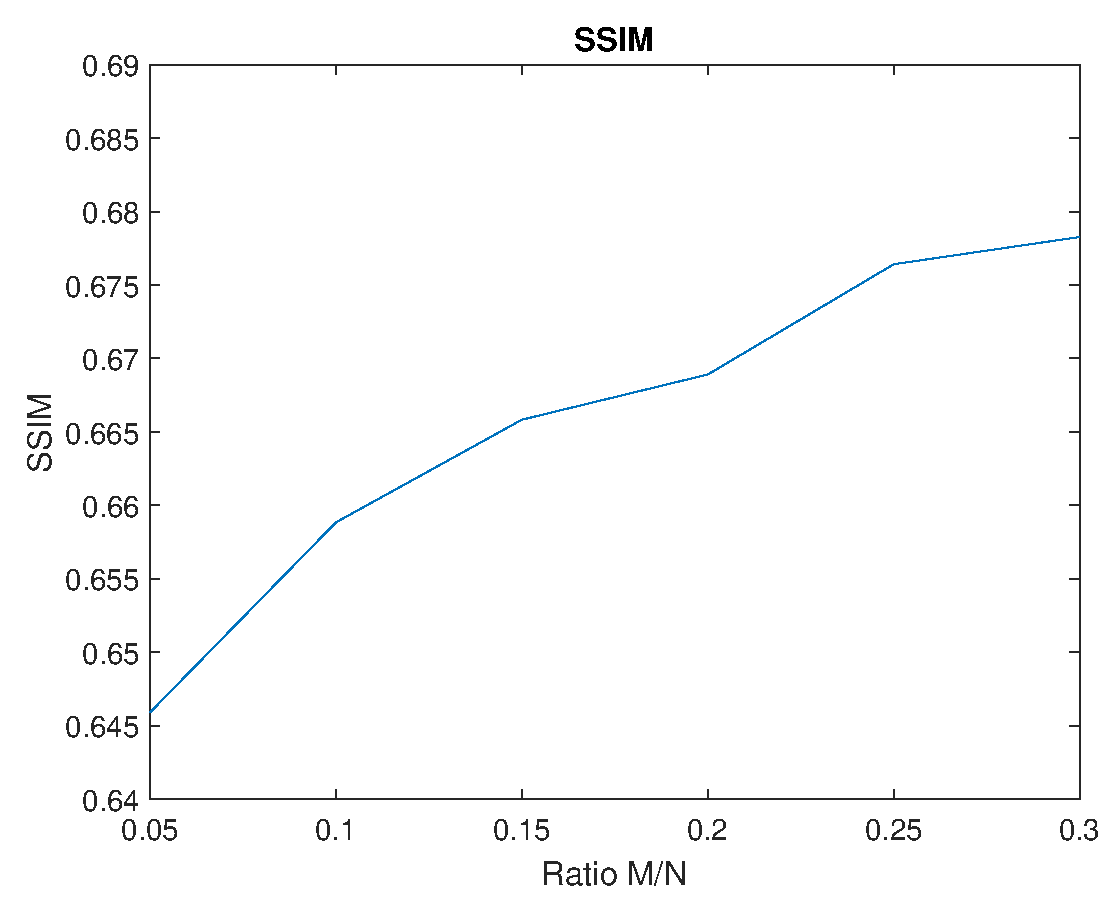
\includegraphics[width=1\textwidth]{result/homo/SSIM_2.eps}
    \subcaption{}
    \label{fig:hom_ssim}
\end{minipage}
    \caption{Signal quality of SPC images compared to reference image. (a) Peak SNR for reconstructed images against reference image. (b) SSIM score for reconstructed images against reference image.}
    \label{fig:hom_score}
\end{figure}

The result shows the same expected result as before with increased quality with increased subsample ratio. An second observation confirms the observation made in section~\ref{sec:measurements}, where the image quality is rapidly improves when increasing subsample ratio to to 15\%, then the improvement rate stagnates. 



\subsubsection{Reconstruction performance Using no reference quality assessment}
\label{sec:SPC_BRISQUE}
In this section the blind quality assessment tool BRISQUE will be used to score the reconstructed images from the SPC. The same algorithm was used on the simulated data where a benchmark was set as a theoretical limit to the reconstructed images.\\[0.1in]     

Each image is evaluated at subsampling rate from $5\%$ to $30\%$ where the result is presented in figure~\ref{fig:brisque_plot}.

\begin{figure}[H]
    \centering
    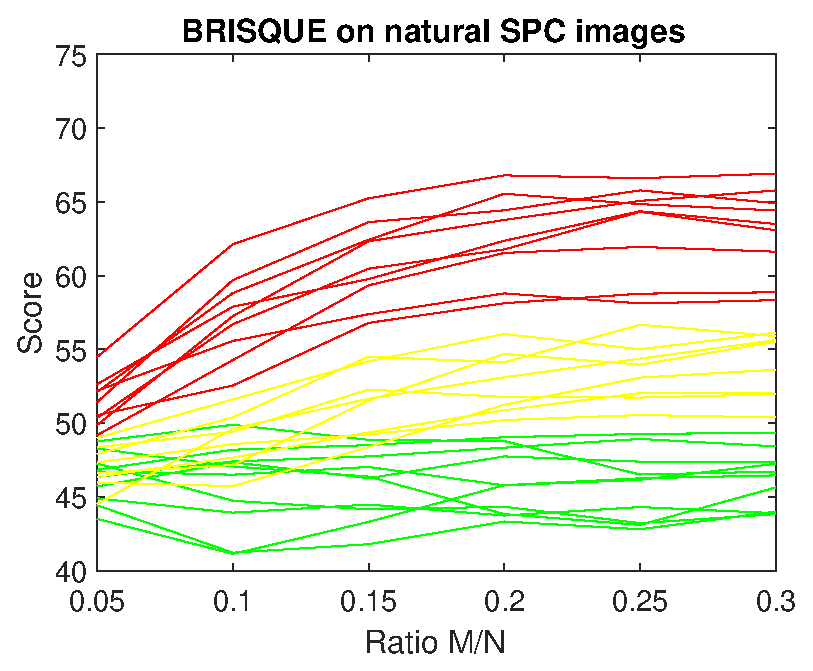
\includegraphics[width = 0.7\linewidth]{result/SPC_NRQA/brisque_spc.eps}
    \caption{BRISQUE score for images reconstructed from the SPC with subsampling ratios from $5\%$ to $30\%$. Each line represent one image and is classified with different colors representing start score at smallest subsampling ratio and general trend when subsampling ratio is increased.}
    \label{fig:brisque_plot}
\end{figure}


As seen in figure~\ref{fig:brisque_plot} each image as been plotted separately, this is because the high variance in the scores and the distinct different trends in the score. Furthermore the images has been classified into three different classes depending on the initial score at 5\% subsampling and the trend when increasing the subsampling ratio\todo{an visually inspecting the images}. The classes has been color coded where:

\begin{itemize}
\item Red means bad score from the first subsampling ratio and a trend line where the score gets worse with more samples.
\item Yellow represent good initial score but the trend line indicates worse image quality when subsampling ratio is increased.
\item Green represent both good initial score and better or stationary score when subsampling ratio is increased. 
\end{itemize}

When studying the BRISQUE score plot in figure~\ref{fig:brisque_plot} from the SPC and comparing to the plot of BRISQUE scores from simulated images in figure~\ref{fig:Brisque_2d} some similarities can be found. The first one is that, the best scores from the SPC has the same score as the simulated images with small or no noise added, which means that the SPC can compare to the benchmark set by the simulated images and thus gives theoretical optimal reconstruction given the measurement matrix and reconstruction algorithm. The second similarity is the trend of the "bad" images which has approximately the same score and trend as the simulated images with larger noise added to the sampled signal. In the last part of this subsection the reconstructed images will first be presented an analyzed followed by a noise analysis to conclude if there is a correlation between noise level and BRISQUE score.\\[0.1in] 


In figure~\ref{fig:good} to \ref{fig:bad} a sample of reconstructed  images are presented from each class with subsampling ratio 30\%. 




\begin{figure}[H]
    \centering
\begin{minipage}[t]{0.245\textwidth}
    
\includegraphics[width=1\textwidth]{result/SPC_NRQA/g64_512_m30.PNG}
    \subcaption{}
    \label{fig:good1}
\end{minipage}
\begin{minipage}[t]{0.245\textwidth}
    
\includegraphics[width = \textwidth]{result/SPC_NRQA/g24_512_m30.PNG}
    \subcaption{}
    \label{fig:good2}
\end{minipage}
\begin{minipage}[t]{0.245\textwidth}
    
\includegraphics[width=1\textwidth]{result/SPC_NRQA/g22_512_m30.PNG}
    \subcaption{}
    \label{fig:good3}
\end{minipage}
\begin{minipage}[t]{0.245\textwidth}
    
\includegraphics[width = \textwidth]{result/SPC_NRQA/g65_512_m30.PNG}
    \subcaption{}
    \label{fig:good4}
\end{minipage}
    \caption{Sample of "good" images corresponding to the green lines in figure~\ref{fig:brisque_plot}.
    (a) and (d) People sitting in the edge of a forest.  (b) Stationary car. (c) Camouflage jackets and a AT-4 anti-tank weapon on the ground.}
    \label{fig:good}
\end{figure}

\begin{figure}[H]
    \centering
\begin{minipage}[t]{0.245\textwidth}
    
\includegraphics[width=1\textwidth]{result/SPC_NRQA/h35_512_m30.PNG}
    \subcaption{}
    \label{fig:half1}
\end{minipage}
\begin{minipage}[t]{0.245\textwidth}
    
\includegraphics[width = \textwidth]{result/SPC_NRQA/h37_512_m30.PNG}
    \subcaption{}
    \label{fig:half2}
\end{minipage}
\begin{minipage}[t]{0.245\textwidth}
    
\includegraphics[width=1\textwidth]{result/SPC_NRQA/h43_512_m30.PNG}
    \subcaption{}
    \label{fig:half3}
\end{minipage}
\begin{minipage}[t]{0.245\textwidth}
    
\includegraphics[width = \textwidth]{result/SPC_NRQA/h62_512_m30.PNG}
    \subcaption{}
    \label{fig:half4}
\end{minipage}
    \caption{Sample of "medium good" images corresponding to the yellow lines in figure~\ref{fig:brisque_plot}.
    (a)  People sitting next to a parking lot. (b) - (d) House facades.}
    \label{fig:half}
\end{figure}

\begin{figure}[H]
    \centering
\begin{minipage}[t]{0.245\textwidth}
    
\includegraphics[width=1\textwidth]{result/SPC_NRQA/b20_512_m30.PNG}
    \subcaption{}
    \label{fig:bad1}
\end{minipage}
\begin{minipage}[t]{0.245\textwidth}
    
\includegraphics[width = \textwidth]{result/SPC_NRQA/b46_512_m30.PNG}
    \subcaption{}
    \label{fig:bad2}
\end{minipage}
\begin{minipage}[t]{0.245\textwidth}
    
\includegraphics[width=1\textwidth]{result/SPC_NRQA/b75_512_m30.PNG}
    \subcaption{}
    \label{fig:bad3}
\end{minipage}
\begin{minipage}[t]{0.245\textwidth}
    
\includegraphics[width = \textwidth]{result/SPC_NRQA/b79_512_m30.PNG}
    \subcaption{}
    \label{fig:bad4}
\end{minipage}
    \caption{Sample of "bad" images corresponding to the red lines in figure~\ref{fig:brisque_plot}.
    (a)  House facade. (b) Crane (Moving clouds in background). (c) Mjärdevi Center facade (Moving clouds reflection in windows). (d) Mjärdevi Center balcony with people having a break (Moving clouds reflection in windows).}
    \label{fig:bad}
\end{figure}

\todo[inline]{Not analyse, What is the difference?}
Lets analyze the images in figure~\ref{fig:good} to \ref{fig:bad} in order to figure out why the BRISQUE score have such high variance and characteristics when increasing the subsampling ratio. The difference between "good" and "half good" images are very subtle, the intensity and visible noise level is a bit more favorable in the "good" images, but as stated in section~\ref{sec:method_eval} the naturalness of the images differ where the "good" images contains more natural shapes and objects. Between the "good"/"half good" and "bad" images there is a more noticeable difference, the images in the "bad" set has more distinct noise and lower over all intensity which most certainly effect the BRISQUE score. Furthermore some of the "bad" image set had movement when sampled which will definitely increase global noise in the images as concluded in section~\ref{sec:Dynamics_in_scene}.\\[0.1in]

When the images was sampled a correlation between the mean signal strength and reconstruction performance was noticed, this is due to the constant background noise from the SWIR photo diode. In figure~\ref{fig:snr} the mean sampled signal strength was plotted against SNR and signal variance calculated from normalizing the sample signal and background noise. The variance was calculated in the same way as the simulated signals in section\ref{sec:simulated_results}.  Each signal has the same corresponding color code from the BRISQUE plot in figure~\ref{fig:brisque_plot}.
 

\begin{figure}[H]
    \centering
\begin{minipage}[t]{0.495\textwidth}
    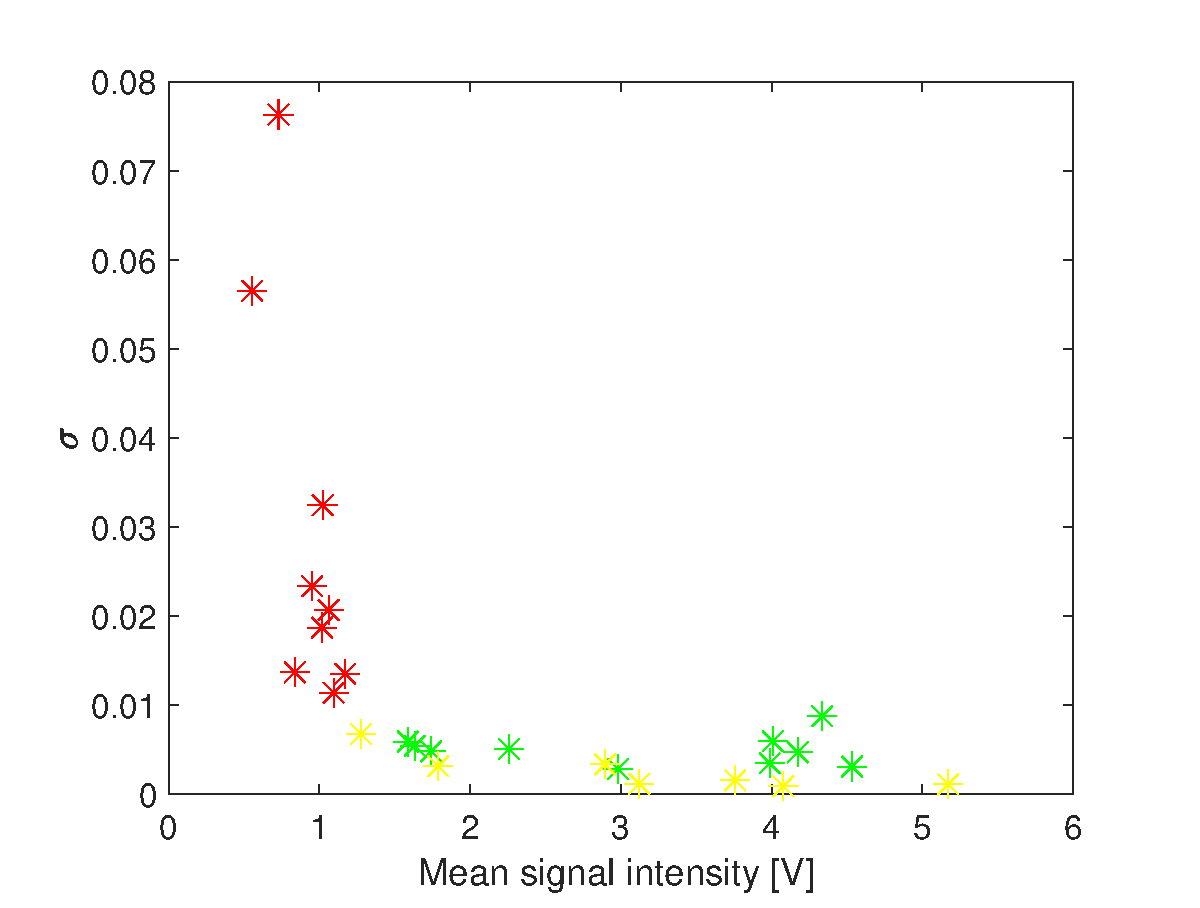
\includegraphics[width=1\textwidth]{result/noise/meanV_sigma.eps}
    \subcaption{}
    \label{fig:snr_v_sigma}
\end{minipage}
\begin{minipage}[t]{0.495\textwidth}
    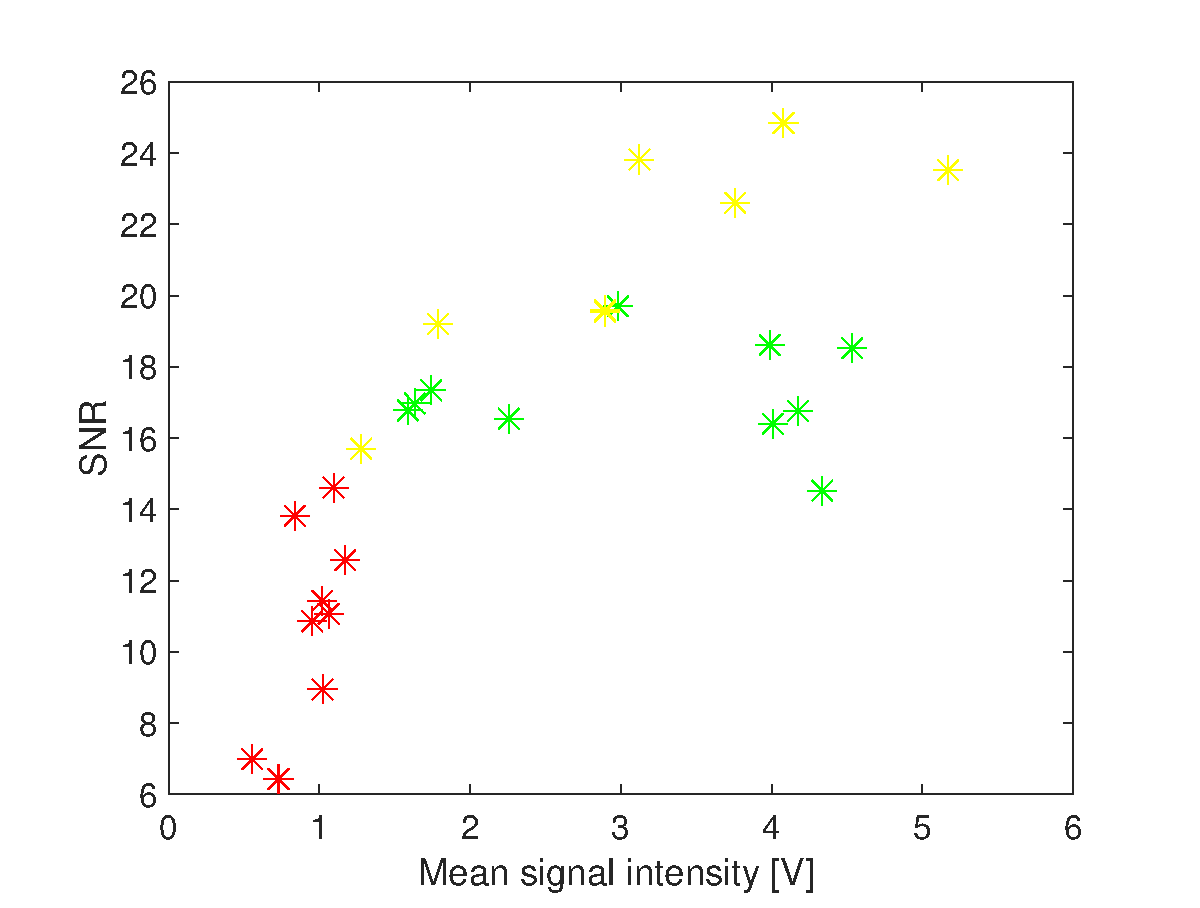
\includegraphics[width = \textwidth]{result/noise/meanV_snr.eps}
    \subcaption{}
    \label{fig:snr_v_SNR}
\end{minipage}
    \caption{Mean sampled signal intensity compared to normalized signal and background noise where each signal has the same corresponding color code from the BRISQUE plot in figure~\ref{fig:brisque_plot}.  (a) Signal intensity against normalized variance from background noise. (b) Signal intensity against SNR from normalized signal and background noise.}
    \label{fig:snr}
\end{figure}

From the two plots in figure~\ref{fig:snr} there are some conclusions that can be made:


\begin{itemize}
\item From both plots in figure~\ref{fig:snr} there is a quite distinct threshold where the signals intensity overcomes the noise level to reconstructed "good" images around 1.2 volt. None of the "good"/"half good" images are below this signal intensity but are mixed over the threshold. 
%The exponential characteristics of the signal to noise ratio given the signal strength means that it should be easy to find a threshold for a given systems background noise.

\item In the plots there are only two signals with higher variance than 0.04 which is the threshold where the the simulated images started to get both worse initial BRISQUE score and worse trend when increasing the subsampling ratio in figure~\ref{fig:Brisque_2d}. This implies that there must be at least one additional factor at play to reduce the image quality in the "bad" set. 


\item There are three red images with almost the same SNR and mean signal intensity as yellow and green images but yields a worse BRISQUE score anyway. This strengthening the statement the there is probably at least on more factor that reduces reconstruction performance.

\item The yellow and green images is mixed for all mean signal strengths which implies that the motive in the images effecting the  BRISQUE score. 

\end{itemize}

\todo[inline]{End klam}


\subsubsection{Luminance Change in scene}
As predicted in section~\ref{sec:Dynamics_in_scene}, dynamics in the scene could result in poor reconstruction performance and an algorithm to suppress this distortion was proposed and tested with good result in the simulated case in section~\ref{sec:dyn_sim}. With a exposure time of just under one minute for the SPC this problem turned out to be constantly present when taking photos at natural scenes outdoors, and the luminace change over time was more complex then the simulated test case. It turned out that the sensor was highly sensitive to luminace change which could not be perceived with the naked eye. This observation should not be unanticipated, the sensor sums up half the scenes light which make the tiniest intensity change for each pixel a large global change. So how did the algorithm hold up for the real application? In figure~\ref{fig:lc_plot} the raw sampled signal is colored red which clearly is not a stationary signal, with the moving average in green and the final improved signal in blue. 

\begin{figure}[H]
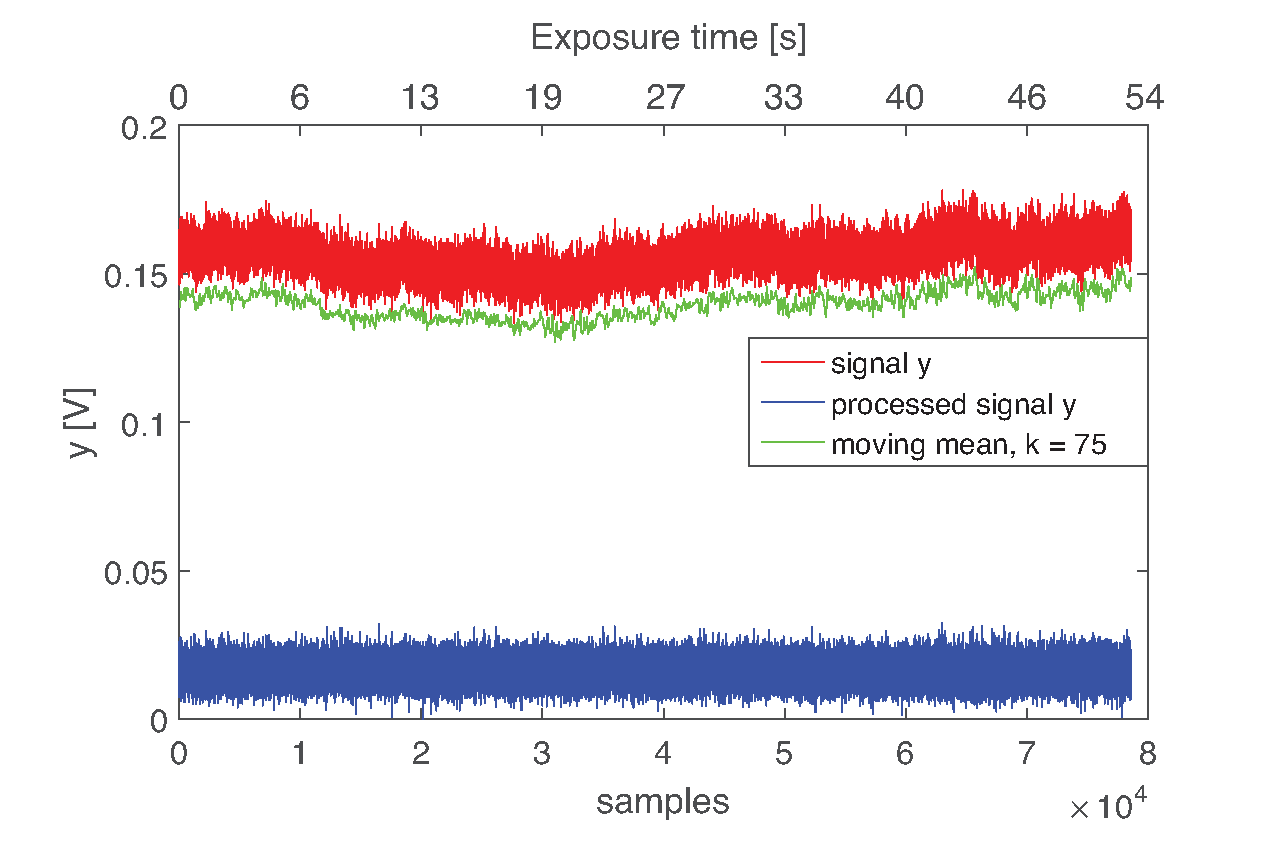
\includegraphics[width = 0.8\linewidth]{result/luminance/li.eps}
	\caption{Sampled signal from SPC with light intensity change and the improved moving mean processed signal.}
	\label{fig:lc_plot}
\end{figure}

As can be seen on the moving average plotted, the intensity change is very fast and can change in matter of a split of a second, "k" which is the number of neighboring samples to calculate the average  was set to 75 to match the fast change which corresponds to a window of 50 milliseconds.\\[0.1in]

In figure~\ref{fig:lc_image} a reconstructed image without the method used and one with the method used is displayed.

\begin{figure}[H]
\begin{minipage}[t]{0.49\textwidth}

\includegraphics[width = 1\linewidth]{result/luminance/24_512_m30.PNG}
	\subcaption{}
	\label{lc_bf}
\end{minipage}
\begin{minipage}[t]{0.49\textwidth}

\includegraphics[width = 1\linewidth]{gfx/car/car_m30.png}
	\subcaption{}
	\label{lc_af}
\end{minipage}
	\caption{Reconstructed images, (a) before and (b) after applying moving mean average method.}
	\label{fig:lc_image}
\end{figure}

As can be seen in the figure, the method produces good result, the image reconstructed without the signal processing has a severe global noise due to the non stationary signal and the reconstruction performance significantly significantly lower. This images is actually one of the images captured in good conditions with strong lighting and mild intensity change overall.


\subsubsection{Edge response}
The edge response is used to comparing the sharpness of cameras and lenses. The edge response from the SPC is compared to a state of the art SWIR camera. Two scenes was captured by the SPC and a conventional SWIR camera containing printed sheath of paper with simple tilted shapes on them, see figure~\ref{fig:mtf_target}. 



\begin{figure}[H]
    \centering
    
\includegraphics[width=0.8\linewidth]{result/mtf/Target.eps}
    \caption{Printed targets with markings where the edge response measurements was performed}
    \label{fig:mtf_target}
\end{figure}

In the resulting images, edge response measurements was gathered from the specified edges in figure~\ref{fig:mtf_target}, with the result from all edges and both images for respective cameras, a mean and standard deviation is calculated. For the SPC, images reconstructed from 5\% to 30\% was tested in order to see if the subsampling ratio effected the MTF result. In figure~\ref{fig:mtf_target_im} the images from the SWIR camera and SPC are presented.

\begin{figure}[H]
    \centering
\begin{minipage}[t]{0.40\textwidth}
    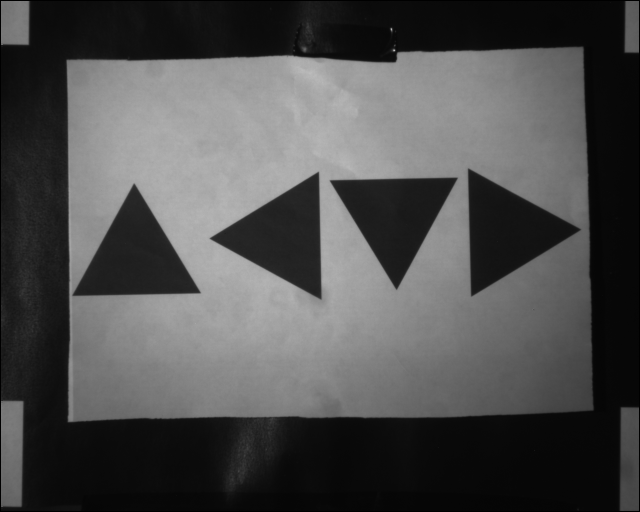
\includegraphics[width=1\textwidth]{result/mtf/swir2.png}
    \subcaption{}
    \label{fig:mtf_s2}
\end{minipage}
\begin{minipage}[t]{0.40\textwidth}
    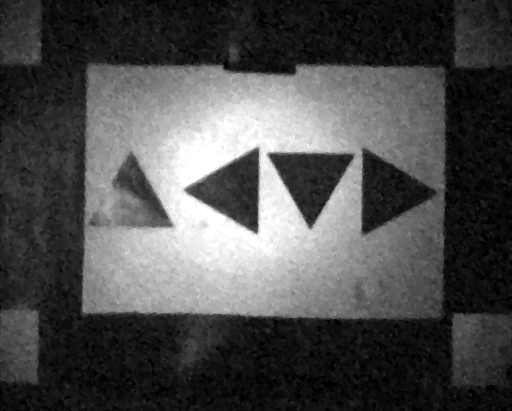
\includegraphics[width=1\textwidth]{result/mtf/spc22.png}
    \subcaption{}
    \label{fig:mtf_spc2}
\end{minipage}
\begin{minipage}[t]{0.40\textwidth}
    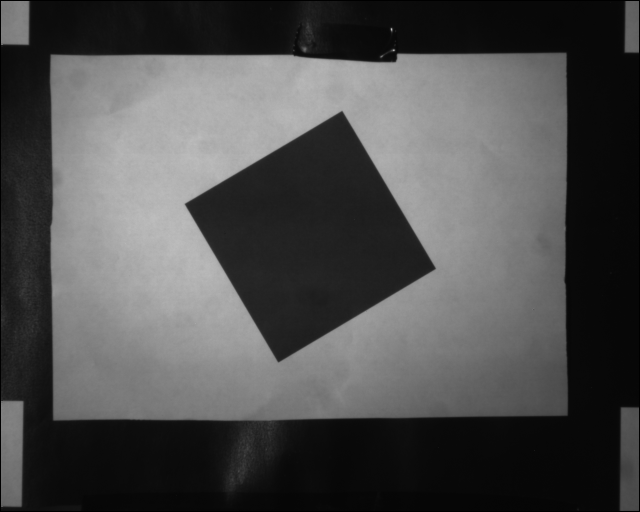
\includegraphics[width=1\textwidth]{result/mtf/swir1.png}
    \subcaption{}
    \label{fig:mtf_s1}
\end{minipage}
\begin{minipage}[t]{0.40\textwidth}
    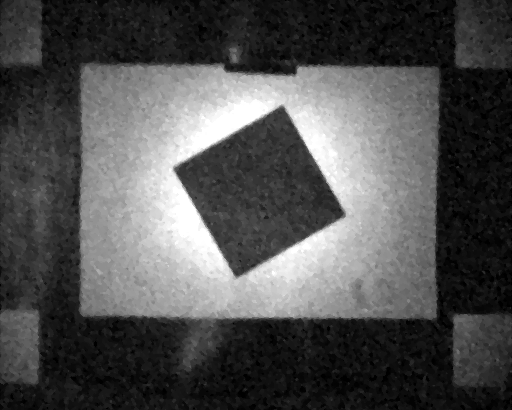
\includegraphics[width=1\textwidth]{result/mtf/spc12.png}
    \subcaption{}
    \label{fig:mtf_spc1}
\end{minipage}
    \caption{SPC and state of the art SWIR camera images. (a) and (c) from the conventional SWIR camera and (b) and (c) captured with the SPC.}
    \label{fig:mtf_target_im}
\end{figure}




The edge response is measured in the distance (pixels) required for a edge to rise from $10\%$ to $90\%$ intensity change. In figure~\ref{fig:rise} the result from the experiment in presented. 

\begin{figure}[H]
    \centering
    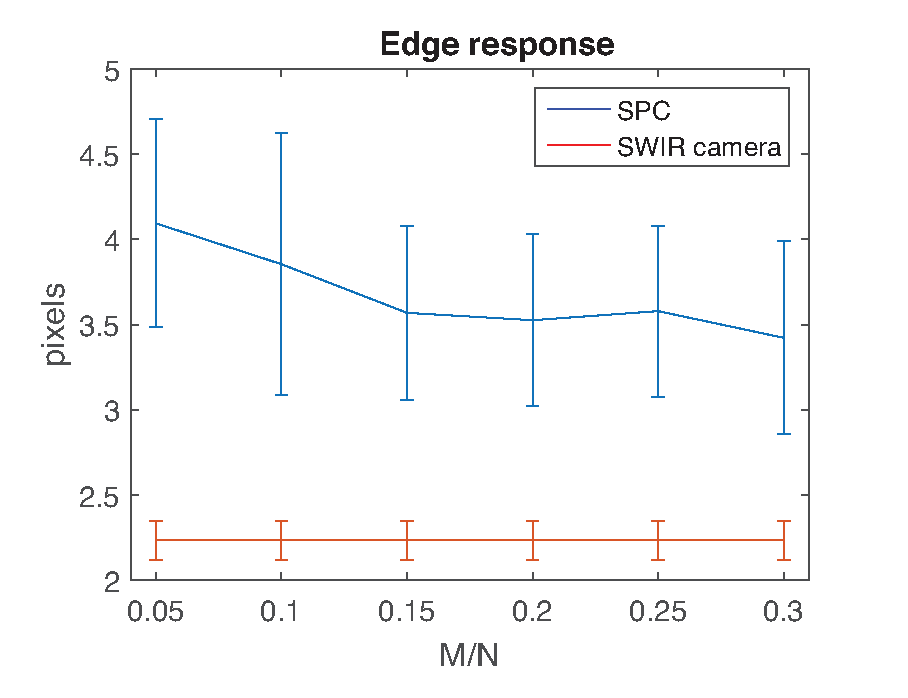
\includegraphics[width=0.7\linewidth]{result/mtf/Rise10_90.eps}
    \caption{Edge response, distance (pixels) to rise from 10-90\% in average for an edge.}
    \label{fig:rise}
\end{figure}

From the plot in figure~\ref{fig:rise}, a clear difference between the SPC and state of the art SWIR camera can be seen, where the conventional SWIR camera has in average half the distance against the SPC images. Some improvement is seen when the subsample ratio is increased, but the standard deviation is almost constant, meaning that the difference between the state of the art SWIR camera and the SPC, in best case only differ about 0.5 pixels, but in the worst case differ about 1.7 pixels and in average 1.2 pixel.

\subsubsection{Number of measurements}
\label{sec:measurements}
From the theory of compressive sensing the number of measurements needed to reconstruct an image is correlated with the sparsity or compressibility of the image, therefore it is hard to give a good estimate of a subsampling ratio needed to obtain a desired quality of the reconstruction. In addition, using a SPC where noise contaminate the signal and the scene may not be completely stationary, the number of measurements needed will increase in proportion to the noise and the change in the scene. In this subsection the minimum subsampling ratio will be presented followed by how the reconstructed image quality is effected by an increese of subsampling ratio.\\[0.1in]


The minimum number of measurements to reconstruct a image where the motive can be recognized is also effected by the factors described, trying to reconstruct an image under the minimum subsampling ratio results in an image with just noise. A survey of the minimum subsampling ratio was performed on all images captured by the SPC in this thesis, and the result ranged from 2\% to 4\% to obtain a recognizable images, in figure~\ref{fig:minimum_fig} a sample of three images with varying minimum subsambling ratios is displayed.


\begin{figure}[H]
\begin{minipage}[t]{0.32\linewidth} %Car
	
\includegraphics[width = 1\linewidth]{result/minimum/24_512_m2.PNG}
	\subcaption{Subsampling ratio 2\%.}
	\label{fig:minimum_car}
\end{minipage}
\begin{minipage}[t]{0.32\linewidth} % Hus
	
\includegraphics[width = 1\linewidth]{result/minimum/37_512_m3.PNG}
	\subcaption{Subsampling ratio 3\%.}
	\label{fig:minimum_house}
\end{minipage}
\begin{minipage}[t]{0.32\linewidth} %Sit
	
\includegraphics[width = 1\linewidth]{result/minimum/64_512_m3.PNG}
	\subcaption{Subsampling ratio 3\%.}
	\label{fig:minimum_forest}
\end{minipage}
	\caption{Varying minimum subsampling ratios to reconstruct sample images captured by the SPC.}
	\label{fig:minimum_fig}
\end{figure}

In the sample images in figure~\ref{fig:minimum_fig} the minimum subsampling ratio varied between 2\% to 3\%, but as can be seen, this is only the minimum subsampling ratio where the motive is barley recognizable, large structure can be identified but detail is lost. In general a subsampling ratio of 5\% has always succeeded to reconstruct a identifiable image with some fine details, moving along this topic the results from higher subsampling ratios is presented.\\[0.1in]

In figure~\ref{fig:subsampling_ratios} three scenes is reconstructed using different subsample ratios ranging from 5\% to 30\%, for each row the subsampling ratio is increased by 5\% and at the top a reference image from a visual camera is presented. What should be expected is increased image quality with increased subsampling ratio, this result can give an perception of which subsampling ratio is good enough for a given purpose, and as can be seen, the increase of subsampling ratio is not linear proportional to the increase in perceived image quality, just like regular image compression.
     

\begin{figure}[H]
\begin{minipage}[t]{0.3\linewidth} %Car
	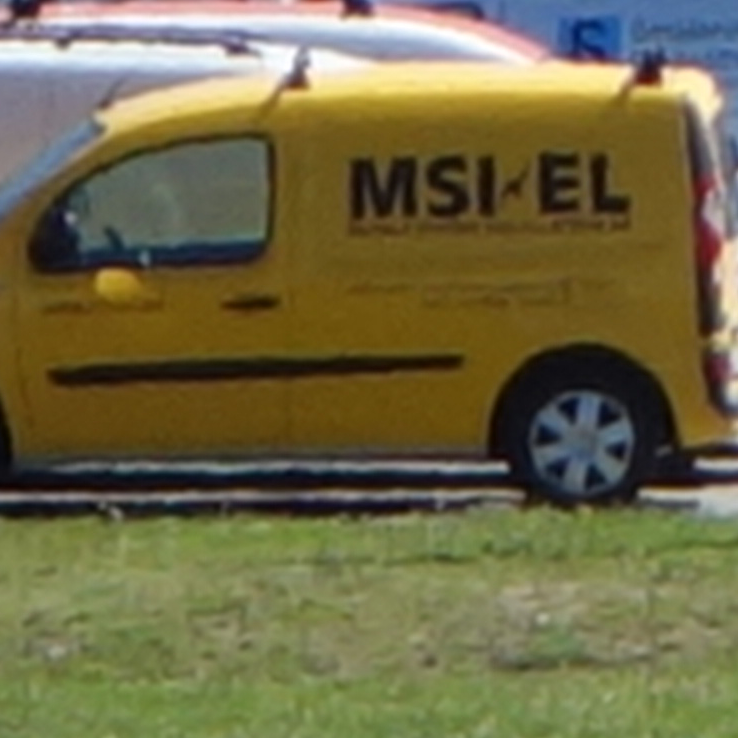
\includegraphics[width = 1\linewidth]{gfx/car/car_org.png}
	%\subcaption{Visual camera image.}
	\label{fig:car_org}
\end{minipage}
\begin{minipage}[t]{0.3\linewidth} % Hus
	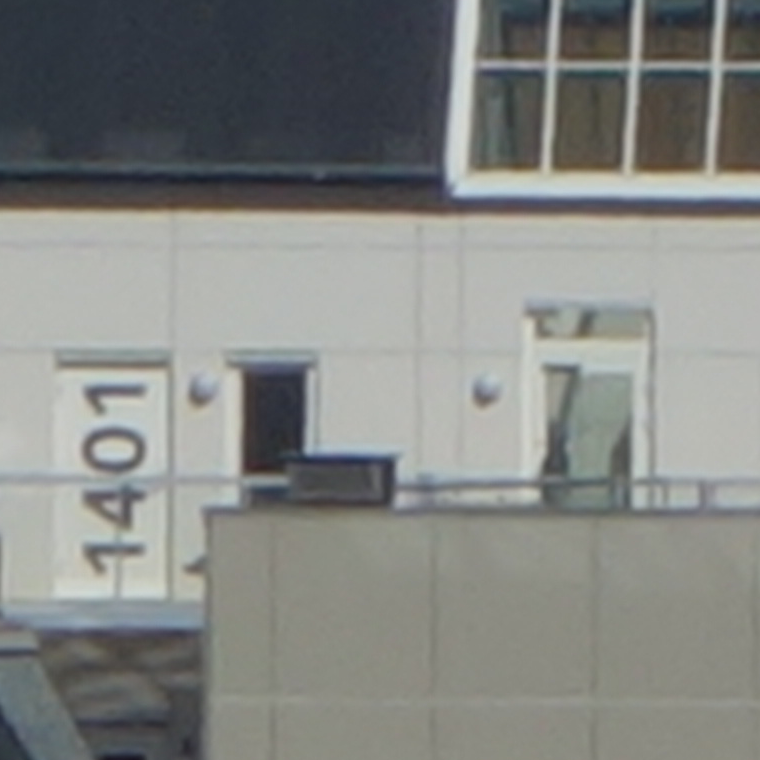
\includegraphics[width = 1\linewidth]{gfx/hus/hus_org.png}
	\subcaption{Visual camera image.}
	\label{fig:hus_org}
\end{minipage}
\begin{minipage}[t]{0.3\linewidth} %Sit
	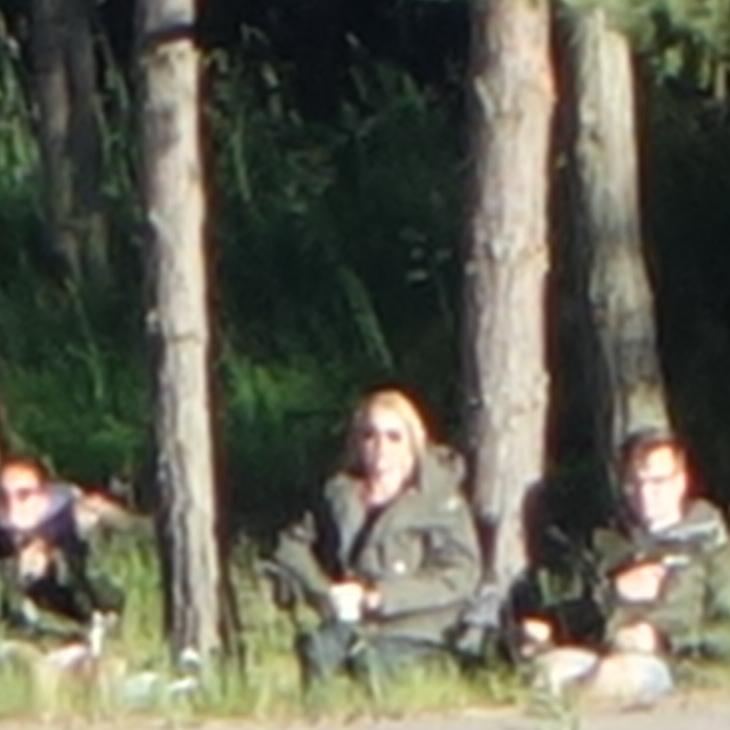
\includegraphics[width = 1\linewidth]{gfx/sit/sit_org.png}
	%\subcaption{}
	\label{fig:sit_org}
\end{minipage}
\begin{minipage}[t]{0.3\linewidth} %Car
	
\includegraphics[width = 1\linewidth]{gfx/car/car_m5.png}
	%\subcaption{Subsampling ratio 5\%}
	\label{fig:car_m5}
\end{minipage}
\begin{minipage}[t]{0.3\linewidth} % Hus
	
\includegraphics[width = 1\linewidth]{gfx/hus/hus_m5.png}
	\subcaption{Subsampling ratio 5\%}
	\label{fig:hus_m5}
\end{minipage}
\begin{minipage}[t]{0.3\linewidth} %Sit
	
\includegraphics[width = 1\linewidth]{gfx/sit/sit_m5.png}
	%\subcaption{}
	\label{fig:sit_m5}
\end{minipage}
\begin{minipage}[t]{0.3\linewidth} %Car
	
\includegraphics[width = 1\linewidth]{gfx/car/car_m10.png}
	%\subcaption{Subsampling ratio 10\%}
	\label{fig:car_m10}
\end{minipage}
\begin{minipage}[t]{0.3\linewidth} % Hus
	
\includegraphics[width = 1\linewidth]{gfx/hus/hus_m10.png}
	\subcaption{Subsampling ratio 10\%}
	\label{fig:hus_m10}
\end{minipage}
\begin{minipage}[t]{0.3\linewidth} %Sit
	
\includegraphics[width = 1\linewidth]{gfx/sit/sit_m10.png}
	%\subcaption{}
	\label{fig:sit_m10}
\end{minipage}
\begin{minipage}[t]{0.3\linewidth} %Car
	
\includegraphics[width = 1\linewidth]{gfx/car/car_m15.png}
	%\subcaption{Subsampling ratio 15\%}
	\label{fig:car_m15}
\end{minipage}
\begin{minipage}[t]{0.3\linewidth} % Hus
	
\includegraphics[width = 1\linewidth]{gfx/hus/hus_m15.png}
	\subcaption{Subsampling ratio 15\%}
	\label{fig:hus_m15}
\end{minipage}
\begin{minipage}[t]{0.3\linewidth} %Sit
	
\includegraphics[width = 1\linewidth]{gfx/sit/sit_m15.png}
	%\subcaption{}
	\label{fig:sit_m15}
\end{minipage}
\end{figure}
\begin{figure}[H]
\ContinuedFloat
\begin{minipage}[t]{0.3\linewidth} %Car
	
\includegraphics[width = 1\linewidth]{gfx/car/car_m20.png}
	%\subcaption{Subsampling ratio 20\%}
	\label{fig:car_m20}
\end{minipage}
\begin{minipage}[t]{0.3\linewidth} % Hus
	
\includegraphics[width = 1\linewidth]{gfx/hus/hus_m20.png}
	\subcaption{Subsampling ratio 20\%}
	\label{fig:hus_m20}
\end{minipage}
\begin{minipage}[t]{0.3\linewidth} %Sit
	\includegraphics[width = 1\linewidth]{gfx/sit/sit_m20.png}
	%\subcaption{}
	\label{fig:sit_m20}
\end{minipage}
\begin{minipage}[t]{0.3\linewidth} %Car
	\includegraphics[width = 1\linewidth]{gfx/car/car_m25.png}
	%
	\label{fig:car_m25}
\end{minipage}
\begin{minipage}[t]{0.3\linewidth} % Hus
	\includegraphics[width = 1\linewidth]{gfx/hus/hus_m25.png}
	\subcaption{Subsampling ratio 25\%}
	\label{fig:hus_m25}
\end{minipage}
\begin{minipage}[t]{0.3\linewidth} %Sit
	\includegraphics[width = 1\linewidth]{gfx/sit/sit_m25.png}
	%\subcaption{}
	\label{fig:sit_m25}
\end{minipage}
\begin{minipage}[t]{0.3\linewidth} %Car
	\includegraphics[width = 1\linewidth]{gfx/car/car_m30.png}
	%\subcaption{Subsampling ratio 30\%}
	\label{fig:car_m30}
\end{minipage}
\begin{minipage}[t]{0.3\linewidth} % Hus
	\includegraphics[width = 1\linewidth]{gfx/hus/hus_m30.png}
	\subcaption{Subsampling ratio 30\%}
	\label{fig:hus_m30}
\end{minipage}
\begin{minipage}[t]{0.3\linewidth} %Sit
	\includegraphics[width = 1\linewidth]{gfx/sit/sit_m30.png}
	%\subcaption{}
	\label{fig:sit_m30}
\end{minipage}
	\label{fig:subsampling_ratios}
	\caption{Reconstructed images captured by the SPC with increasing subsampling ratios. First row showing a reference visual spectrum image followed by SPC images reconstructed with 5\% from top then increased subsampling ratio by 5\% for each row to 30\% on the last row.} 
\end{figure}

The are a few thinks that can be noted in the images in figure~\ref{fig:subsampling_ratios}, 

\begin{itemize}
\item the reconstructed images behave as expected, when the subsample ratio increases the image quality increases. 

\item Already at 5\% subsampling ratio the scene can be properly identified unlike the case in minimal subsamples ratio. The images has some artifacts that can be linked to the reconstruction algorithm, the images looks like the made of small patches.

\item Between 10-15\% the finer details start to appear, like the gap between the panels in the facade, the text on the car and door are getting sharper and the structure of the faces start to appear.

\item As stated before, the image quality does not increase at the same rate as the subsampling ratio, this is most noticeable when increasing the subsampling ratio above 15\%. The improvement after 15\% is not as easy to spot as from the increments before, but they can be found in the details. 
\end{itemize}



 





